\documentclass{article}

\usepackage[margin=1in]{geometry}
\usepackage{tikz}
\usepackage{environ}

\makeatletter
\newsavebox{\measure@tikzpicture}
\NewEnviron{scaletikzpicturetowidth}[1]{%
  \def\tikz@width{#1}%
  \def\tikzscale{1}\begin{lrbox}{\measure@tikzpicture}%
  \BODY
  \end{lrbox}%
  \pgfmathparse{#1/\wd\measure@tikzpicture}%
  \edef\tikzscale{\pgfmathresult}%
  \BODY
}
\makeatother

\begin{document}
The below figures illustrate the Round-robin algorithm with arbitrary data:
\begin{minipage}[c]{0.4\textwidth}
  \centering
  \begin{tabular}{|c c c|}
    \hline
    Process & Arrival time & Execution time \\ [0.5ex]
    \hline\hline
    0 & 1 & 5 \\
    1 & 1 & 3 \\
    2 & 2 & 8 \\
    3 & 3 & 8 \\ [1ex]
    \hline
  \end{tabular}
\end{minipage}
\begin{minipage}[c]{0.4\textwidth}
  \centering
  \begin{scaletikzpicturetowidth}{\pagewidth}
    \begin{tikzpicture}[xscale=1]
      \draw [fill=gray] (0,0) rectangle (5,2);
      \node at (2.5,1) {P0};
      \draw [-] (0,0) -- (0,-2);
      \node [below] at (0,-2) {0};
      \draw [fill=gray] (5,0) rectangle (13,2);
      \node at (9,1) {P1};
      \draw [-] (5,0) -- (5,-2);
      \node [below] at (5,-2) {5};
      \draw [fill=gray] (13,0) rectangle (29,2);
      \node at (21,1) {P2};
      \draw [-] (13,0) -- (13,-2);
      \node [below] at (13,-2) {8};
      \draw [fill=gray] (29,0) rectangle (51,2);
      \node at (40,1) {P3};
      \draw [-] (29,0) -- (29,-2);
      \node [below] at (29,-2) {16};
      \draw [-] (51,0) -- (51,-2);
      \node [below] at (51,-2) {22};
    \end{tikzpicture}
  \end{scaletikzpicturetowidth}
\end{minipage}
\end{document}
